\chapter{PathObjects for Squeak/Smalltalk}
\label{c:implementation}
To validate the applicability of the \textsc{PathObjects} concept, we put it into practice in the form of a prototype for the Squeak/Smalltalk environment.
This chapter describes the implementation of this prototype, which also served as a basis for the performance analysis and user evaluation (cf. Chapter \ref{c:discussion}).
Section \ref{s:ImplementationPrototype} shows how the single concepts - namely navigation, exploration, focusing, and information layers - are realized.
The subsequent sections present technical implementation details.
Section \ref{s:ImplementationTracing} describes how the lightweight tracing approach works.
Furthermore, it explains the necessary extensions of the \textsc{PathTools} framework that allow us to reconstruct object interactions and referential relationships.
Finally, Section \ref{s:ImplementationLayouting} illustrates how \textsc{PathObjects} traces can be mapped to graphs, and how this circumstance is exploited to arrange objects and to route messages with the help of \textsc{Graphviz}.

\section[Prototypic Implementation]{Prototypic Implementation%
\sectionmark{Prototype}}
\sectionmark{Prototype}
\label{s:ImplementationPrototype}

\begin{figure}
	\centering
	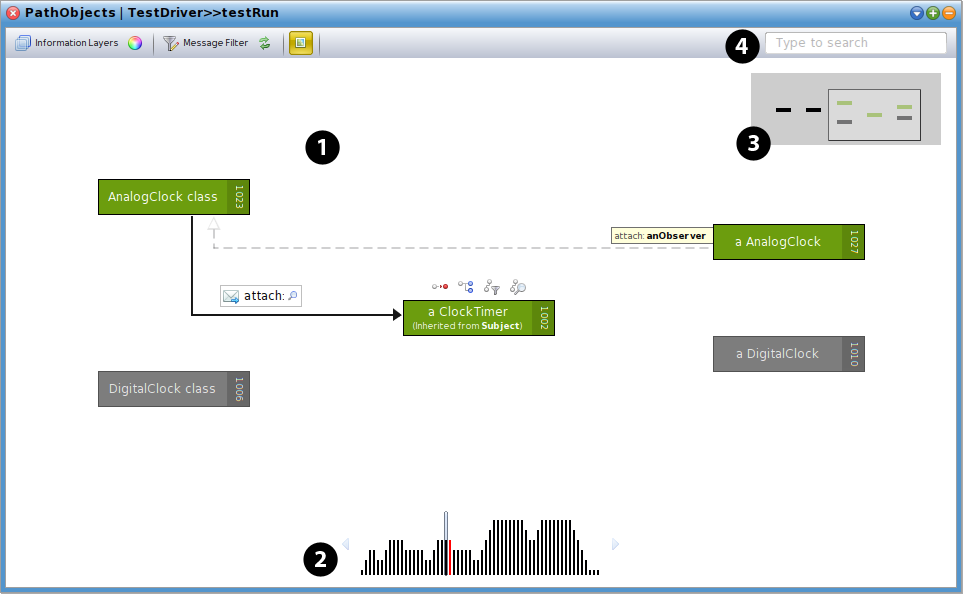
\includegraphics[width=1\textwidth]{../images/04-ImplMainWindow}
	\caption[TOC Caption]{Foobar}
	\label{fig:ImplementationMainWindow}
\end{figure}

\subsection{Exploration}

\begin{figure}[tb]
	\centering
	
	\begin{subfigure}[b]{0.90\textwidth}
		\centering
		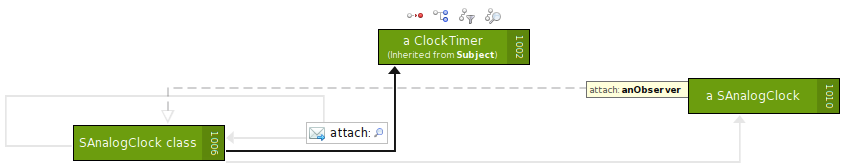
\includegraphics[width=\textwidth]{../images/04-ImplExploration1}
		\caption[Foo]{}
		\label{fig:ImplementationExplorationBasic}
	\end{subfigure}
	
	\caption[Foo]{Foo}
	\label{fig:ImplementationMinimap}
\end{figure}

Figure \ref{fig:ImplementationExplorationBasic} shows the basic visualization of object interactions that allows developers to explore the behavior of a system.
Objects that are involved in the current step of the execution are emphasized through green background color (in the given example, all shown objects are involved).
The current message send is indicated through a black arrow, and the previous three steps are drawn in lighter colors.
The example shows that the class \inlinecode{SAnalogClock} sends the \inlinecode{attach:} message to an instance of \inlinecode{ClockTimer}.
The argument of the \inlinecode{attach:} message is an instance of \inlinecode{SAnalogClock}.
This is illustrated through the yellow flag that is attached to the object.
To clarify the role of an object in the current step even further, this indicator also shows the name the underlying method defines for this argument, namely \inlinecode{anObserver}.

The developer can explore the implementations of the current message and of the context in which this message is sent through clicking on the icon left of the message name.
The icon on the right of the message name allows to directly explore the state of the argument.
The icons that are shown above the clock timer instance are a context sensitive menu that is displayed when the developer hovers an object.
It allows to take further actions regarding the respective object.
From left to right, these are toggling state tracking, toggling outbound reference tracking, setting of a quick filter, and execution of a quick search.
All of these features are explained in the following.

\subsubsection{State Exploration}

\begin{figure}[b]
	\centering
	
	\begin{subfigure}{0.45\textwidth}
		\centering
		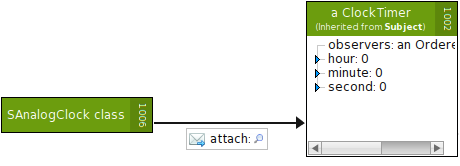
\includegraphics[width=\textwidth]{../images/04-ImplExplorationState1}
		\caption[Foo]{}
		\label{fig:ImplementationExplorationState1}
	\end{subfigure}
	\quad
	\begin{subfigure}{0.45\textwidth}
		\centering
		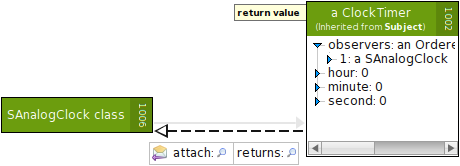
\includegraphics[width=\textwidth]{../images/04-ImplExplorationState2}
		\caption[Foo]{}
		\label{fig:ImplementationExplorationState2}
	\end{subfigure}
	
	\caption[Foo]{Foo}
	\label{fig:ImplementationExplorationState}
\end{figure}

Developers can toggle state tracking through an object's context menu.
As long as state tracking is enabled, the state of an object is expanded below the object header and automatically updated whenever the developer steps to a different point of the execution history.

Figure \ref{fig:ImplementationExplorationState} gives an example with the aid of the process of adding observers to the subject.
In Figure \ref{fig:ImplementationExplorationState1}, the state of the system is shown before the \inlinecode{attach:} message has been processed.
\inlinecode{SAnalogClock class} is the sender of this message, and an instance of \inlinecode{SAnalogClock} is the argument of this message (but not shown in the figure).
State tracking is enabled for the clock timer instance, and the state explorer shows that no observers are currently registered and that the hour, minute, and second attributes are equal to \inlinecode{0}.
Figure \ref{fig:ImplementationExplorationState2} depicts the state of the system after the \inlinecode{attach:} message has been processed, or respectively after the developer took a step forward in the execution history.
The message label now has an additional field to explore the return value.
The latter turns out to be the clock timer instance, and this fact is also clarified through the role indicator that is attached to the object.
But the most important change is visible in the state explorer.
It can be seen that the collection of observers now has one entry, and this entry is the instance of \inlinecode{SAnalogClock} that has been passed as argument.

\subsubsection{Reference Exploration}
\textsc{PathObjects} not only allows developers to track object state changes, but also to chase outbound pointers of specific objects.
The mechanism works similar to the state exploration described above.
Developers can toggle reference exploration through the context menu of an object.
When enabling exploration, the developer is prompted to select a color.
This selection will then be used as background color of all referenced objects.
The current outbound pointers are collected when stepping through the execution history, and the background colors of referenced objects are updated accordingly.
This allows developers to get an insight which other objects a specific one references, when these references are gained, and when they are released.


\subsection{Navigation}
\label{ss:ImplementationNavigation}
The implementation of the \textsc{PathObjects} concept for Squeak/Smalltalk offers three features that assist developers in navigating through an execution history.
First, the timeline gives an overview of all steps of the execution, or respectively the message sends and returns.
Second, the mini-map displays which objects are currently in the viewport, and which other objects also occur during the execution.
Third, the search bar allows developers to find classes, message sends, or specific instances

\subsubsection{Timeline}

\begin{figure}[tb]
	\centering
	
	\begin{subfigure}[b]{0.45\textwidth}
		\centering
        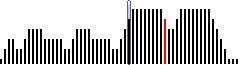
\includegraphics[width=\textwidth]{../images/04-ImplTimeline1}
        \caption[Default View]{}
		\label{fig:ImplementationTimelineDefault}
	\end{subfigure}
	\quad
	\begin{subfigure}[b]{0.45\textwidth}
		\centering
		
\includegraphics[width=\textwidth]{../images/04-ImplTimeline2}
		\caption[Search Result Highlighting]{}
		\label{fig:ImplementationTimelineSearch}
	\end{subfigure}
	\quad
	\begin{subfigure}[b]{0.45\textwidth}
		\centering
		
\includegraphics[width=\textwidth]{../images/04-ImplTimeline3}
		\caption[Differing Metrics Applied to Item Height and Color]{}
		\label{fig:ImplementationTimelineMetrics}
	\end{subfigure}
	
	\caption[Variations of the Timeline View]{Three variations of the timeline view that show the exact same execution history; in each case, the current step is highlighted and the according return point is marked in red.
		a) Default view with mapping of stack depth to item height.
		b) Search result highlighting.
		c) Differing metrics applied to item height and item color.
	}
	\label{fig:ImplementationTimeline}
\end{figure}

Figure \ref{fig:ImplementationTimeline} shows examples of the timeline view.
Each bar represents a step of the execution history, or respectively either a message send or the return from a message send.
The alignment along the horizontal axis corresponds to the chronological order of appearances.
The current step is marked with a blue overlay, and the corresponding send or return step is marked in red.
Developers can use the timeline to navigate through the execution history by either selection a specific step, by using the keyboard's left and right arrows, or by clicking the arrows that are displayed alongside the timeline.

All three examples in Figure \ref{fig:ImplementationTimeline} show the exact same execution history at the exact same point of the execution.
Figure \ref{fig:ImplementationTimelineDefault} represents the default configuration of the timeline view.
In this case, the height of the single timeline items corresponds to the depth of the call stack.
However, the concept of information layers (cf. \ref{??}\todo{cite}) allows to map arbitrary metrics to this dimension of the diagram.
Figure \ref{fig:ImplementationTimelineSearch} shows how search results are highlighted within the timeline.
In the depicted example, the developer performed a search for occurrences of the \inlinecode{attach:} message.
Two matches are found, whereby each consists of a send and a returns step.
These occurrences correspond to the registration of the analog and digital clock instances at the clock timer.
Figure \ref{fig:ImplementationTimelineMetrics} illustrates the usage of information layers in conjunction with the timeline view.
The height of the items now no longer represents the stack depth, but the number of variable accesses in each method.
The color of the items indicates the lines of code of each message.
One can see that the current step is the one with by far the most variable accesses.
Furthermore, the visualization indicates that most methods have an acceptable length, with the exception of the method that is the implementation of the selected message.

\subsubsection{Minimap}

\begin{figure}[tb]
	\centering
	
	\begin{subfigure}[b]{0.45\textwidth}
		\centering
		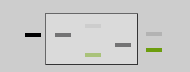
\includegraphics[width=\textwidth]{../images/04-ImplMinimap1}
		\caption[Foo]{}
		\label{fig:ImplementationMinimapDefault}
	\end{subfigure}
	\quad
	\begin{subfigure}[b]{0.45\textwidth}
		\centering
		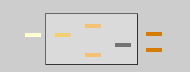
\includegraphics[width=\textwidth]{../images/04-ImplMinimap2}
		\caption[Foo]{}
		\label{fig:ImplementationMinimapMetric}
	\end{subfigure}
	
	%\vspace{0.5cm}	
	%
	%\begin{subfigure}[b]{0.45\textwidth}
	%	\centering
	%	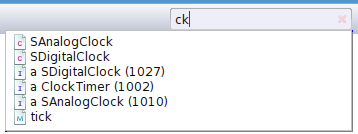
\includegraphics[width=\textwidth]{../images/04-ImplSearch}
	%	\caption[Foo]{}
	%	\label{fig:ImplementationSearch}
	%\end{subfigure}
	%
	\caption[Foo]{Foo}
	\label{fig:ImplementationMinimap}
\end{figure}

Contrary to the timeline, which allows to explore the chronological dimension of execution traces, the mini-map supports developers in the navigation of the spatial dimension of object interaction diagrams.
It shows all objects that occur in a trace at a glance and allows to jump to any part of the canvas through mouse interactions.
Furthermore, it depicts which part of the canvas is currently displayed through a miniaturized viewport indicator.
Figure \ref{fig:ImplementationMinimapDefault} depicts the default mini-map visualization.
All objects that are involved in the current step, either as sender, receiver, or argument of a message, are marked in green.
Objects that already occurred in the past of the execution history are depicted as black boxes.
Objects that did not occur up to the current step but will occur in future steps are marked in light gray.
Figure \ref{fig:ImplementationMinimapMetric} represents an example how information layers can be applied to the mini-map.
In this case, the fan-in metric is mapped to the color of the object's representatives.
The heated-object scale indicates few received messages with light colors and the percipience of many messages in dark colors.
One can see that one object, namely the clock timer, receives more messages than any other object in this trace.

\subsubsection{Search}
The search bar (cf. Figure \ref{fig:ImplementationSearch}) allows developers to find specific entities of interest.
To simplify the process, entities that match a search term are shown and updated as the developer types.
The search functionality supports two different operational modes, namely precise and fuzzy search.
Fuzzy search performs a simple substring matching of the given input, and will return any class instance, class, or message whose name partly or fully matches the given search term.
For instance, this mode makes it possible to find all occurrences of instances of a specific class, by searching for \inlinecode{a ClassName} and omitting the object identifier, which as a matter of fact is part of an object name.
The precise mode, which is enabled as soon as the developer selects an entry from the list of suggested results, allows to search for specific classes, class instances, or messages.
For instance, this allows to search for all occurrences of a specific class.
This would not be possible with fuzzy search alone, since all instances of a class would always also match the search term and would thus lead to a cluttered search result.
As pointed out before, search results are indicated by highlighting timeline items (cf. Figure \ref{fig:ImplementationTimelineSearch}).

\subsection{Focusing}
\subsubsection{Message Filter}
\subsubsection{Object Filter}

\subsection{Information Layers}
\label{ss:ImplementationLayers}

\begin{figure}[tb]
	\centering
	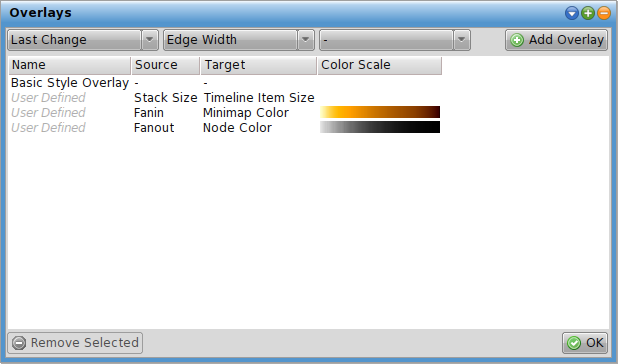
\includegraphics[width=0.7\textwidth]{../images/04-ImplOverlays}
	\caption[Foo]{}
	\label{fig:ImplementationLayers}
\end{figure}

Information layers allow developers to project arbitrary metrics to various dimensions of \textsc{PathObjects} diagrams.
The dialog that allows to configure information layers is shown in figure \ref{fig:ImplementationLayers}.
New layers can be configured with the help of three selection boxes.
First, developers select a metric they wish to visualize.
The second box is then populated with all diagram dimensions the selected metric can be mapped to.
If a dimension is selected that requires the definition of a color scale, this scale can be selected from the third list, which can be ignored otherwise.
In the depicted example, the developer selected to visualize which methods have been changed last, and wishes to display this information with the help of the width of the edges that represent message sends.

The list filling the center of the dialog shows layers that are currently active.
For instance, one user-defined layer maps the \textsc{Fanin}-metric to the color of objects on the mini-map.
Another layer maps the \textsc{Fanout}-metric to the background color of objects, and uses a different color scale for this purpose.
Examples how such layers affect the visualization of various diagram dimensions already have been given in the previous sections (cf. Figures \ref{fig:ImplementationTimelineMetrics}, \ref{fig:ImplementationTimelineMetrics}).

The metrics that are currently supported are listed in Table x and related to the diagram dimensions they can be applied to.
However, the supported metrics as well as the dimensions these metrics can be mapped to constitute an extension point of \textsc{PathObjects}.
The implementation of metrics follow the strategy pattern.
For instance, if a new metric should be added that measures the main memory consumption of single objects, one would have to implement a subclass that lazily executes the test case under observation, performs the required measurements, and returns the measured values for specific objects on demand.
This new metric then could automatically be mapped to any dimension that is suitable to visualize object metrics.

\begin{figure}[tb]
	\centering
	\footnotesize
	\begin{subfigure}[t]{0.45\textwidth}
		\begin{tabular}{ll}
		\toprule[1.5pt]
		Message Metrics		& Dimensions 			\\
		\midrule
		Complexity			& Edge Color 			\\
		Last Change			& Edge Width			\\
		Lines of Code		& Timeline Item Color	\\
		Runtime Profiling	& Timeline Item Height	\\
		Stack Size			&						\\
		Variable Accesses	&						\\
		\bottomrule[1.5pt]
		\end{tabular}
	\end{subfigure}
	\qquad
	\begin{subfigure}[t]{0.45\textwidth}
		\begin{tabular}{ll}
		\toprule[1.5pt]
		Object Metrics		& Dimensions 			\\
		\midrule
		\textsc{Fanin}		& Mini-Map Color		\\
		\textsc{Fanout}		& Object Color			\\
		\textsc{Faninout}	& Object Width			\\
							& Object Height			\\
		\bottomrule[1.5pt]
		\end{tabular}
	\end{subfigure}
\caption[Test Subjects]{Scale of the software systems that served as a basis for the performance evaluation.}
\label{t:EvaluationProjects}
\end{figure}


\section{Data Acquisition}
\label{s:ImplementationTracing}
This section describes how the data required for the reconstruction of object interactions is gathered.
The basic prerequisite is that objects can be distinguished and identified.
Since the Squeak image does not offer an adequate functionality, the strategy that was applied to solve this issue is depicted in Section \ref{ss:ImplementationTracingIdentification}.
Section \ref{ss:ImplementationTracingApproach} describes how the tracing approach works.
Finally, Section \ref{ss:ImplementationTracingReferences} shows how the tracking and mapping of outbound object pointers are implemented.

\subsection{Identification of Objects}
\label{ss:ImplementationTracingIdentification}
The fundamental requirement for the reconstruction of object interactions from traces is that object instances can be identified unambiguously.
Unfortunately, the Squeak image does not provide such a functionality out of the box.
Though objects do have an \inlinecode{identityHash} attribute, the value of this attribute is neither unique nor stable \cite{goldberg_smalltalk-80:_1983}.
In the virtual machine we used, it is derived from the least significant bits of the object pointer which is managed by the virtual machine and represents the object's address in main memory.
Hence, the value of the object pointer and thus the value of the \inlinecode{identityHash} are subject to change during garbage collection, which may cause objects to be moved in main memory.
Furthermore, since the \inlinecode{identityHash} uses only the 12 least significant bits, there is no guarantee that two objects that are not referentially equal cannot share a common hash value \cite{goldberg_smalltalk-80:_1983}.

The Squeak image does not offer a convenient way to access the object pointer, which could serve as unique identifier for objects.
There are workarounds that would allow to determine its value, but since this value still is subject to change during a tracing run due to the reasons pointed out above, it would require to disable garbage collection during this time span.
This could have undesired side effects, like excessive memory consumption or slow execution speeds due to increased memory allocation effort.

For these reasons, we chose a different approach that allows us to generate unique, stable identifiers for objects.
It exploits the fact that that a comparison for referential equality provided by the \inlinecode{==} method will always yield the correct result.
It returns true if the two objects have the same object pointer, and false otherwise.
Squeak provides a \inlinecode{WeakKeyIdentityDictionary} that has two beneficial properties for our use case.
First, it uses \inlinecode{==} comparison to test dictionary keys for equality.
That means that when using the objects that occur during tracing runs as keys, it is guaranteed that no two referentially distinct objects will be identified as the same key, and an object will always be mapped to the same key once it is present in the dictionary.
The second property is that it uses weak references to manage keys, which implicates that garbage collection of an object is not suspended by the fact that it is used as key in such a dictionary.

Consequently, this allows us to use objects occurring during tracing runs as keys, without interfering with the test execution.
Identifiers can be assigned to objects as values of the dictionary.
Thus, it is guaranteed that one object will always be mapped to the same identifier.
To ensure that no identifier is assigned to two referentially different objects, it is sufficient to use a continuously incrementing integer counter when assigning new identities, or respectively when adding new entries to the dictionary.

Since we presuppose that test cases are strictly deterministic (cf. Section \ref{s:DiscussionLimitations}), this strategy results in another benefit.
Namely, objects will always be assigned the same identifier in different tracing runs, since the identifier is only dependent on the chronological order in which objects occur in a trace.
In other words, to stick to the observer example, the instance of \inlinecode{DigitalClock} will always be assigned with the identifier \inlinecode{27} no matter how often the test is executed, since it is the 27th object that occurs in the trace.
This is an important property and prerequisite for the tracing and mapping of outbound object pointers (cf. Section \ref{ss:ImplementationTracingReferences}).

The current implementation constructs a new dictionary of identifiers for each test execution.
But it would also be possible to share identifiers of long living objects like classes across all tracing runs, if a global dictionary were used.
However, we are unaware of a use case that could exploit this possibility, and additional measures would be required to ensure the property described in the previous paragraph.
For these reasons, we favored trace-local over global identity generation.

\subsection{Extensions of the Tracing Framework}
\label{ss:ImplementationTracing}
In order to be suitable for the purposes of \textsc{PathObjects}, the tracing framework provided by \textsc{PathTools} had to be extended in two places.
First, a custom \inlinecode{MethodWrapper} had to be implemented that collects the information required for the reconstruction of object interactions.
For each wrapped executed method, this specialized wrapper reports integer identifiers of the receiving object, of the method arguments, and of the return value to the tracer.
Thereby, argument objects are flattened.
That means that if collections of objects are used as arguments, the identifiers of the objects contained in a collection are reported in addition to the identifier of the collection object itself.
Note that an identifier for the sender of a message is not captured, since it would require the expensive operation of stack inspection.
However, this information can be easily reconstructed from the tree structure of the traces, since the sender of a message is identical to the parent element of a call node in the call tree.

The second extension that had to be made is the implementation of a custom \inlinecode{Tracer} that provides some functionality required by our method wrappers and for additional refinement runs.
It provides an implementation of our object identification approach (cf. Section \ref{ss:ImplementationTracingIdentification}) that is used by the method wrappers to generate unique and stable identifiers for objects that occur during tracing.
Furthermore, it provides entry points for the exploration of outbound object references, and is responsible for the execution of refinement runs that are necessary to collect this information (cf. Section \ref{ss:ImplementationTracingReferences}).

\subsection{Reference Tracing}
\label{ss:ImplementationTracingReferences}
Outbound object pointers - or in other words the set of objects a specific object references - can be determined with the help of  \inlinecode{Object>>outboundPointers}.
However, this method returns only the set of directly referenced objects.
For example, if an instance of \inlinecode{Subject} administers a collection of observers, it would return only the collection object itself, but not the observer objects contained in this collection.
Undoubtedly, this is the technically correct behavior.
But for our purposes it seems more suitable to return those indirectly referenced objects along with the actual references. 
More often than not, this is the actually relevant information for a developer.
Therefore, we decided to flatten the objects returned by \inlinecode{outboundPointers}, and generate identifiers as depicted in Section \ref{ss:ImplementationTracingIdentification} for the resulting objects.
Thus, objects that are wrapped in collections are included when a developer queries the outbound references of a specific object.

Unfortunately, the collection of object references is an expensive operation in two respects.
First, a call of \inlinecode{outboundPointers} is time consuming and thus could slow down the tracing process significantly.
Second, the amount of collected data could grow rapidly if all outbound pointers of all involved objects were collected up-front.
For these reasons, we decided to implement the tracking of object references with the help of refinement runs.
As soon as the user selects an object for reference tracing, the outbound pointers of this object are collected whenever the user steps to another part of of the execution history.
The respective referenced objects are highlighted with a user-defined background color.

As pointed out in Section \ref{ss:ImplementationTracingIdentification}, objects will always be associated with the same identifier in repeated test executions.
This fact is exploited to map the references that are returned from refinement runs to the objects of the current trace.
However, to guarantee that the identifiers from the refinement runs correspond to the identifiers from the shallow analysis run, both executions have to be identical in terms of the tracing code that is executed.
Hence, it is not sufficient to instrument only the method that represents the current step of the execution history.
It is important that the method wrappers request identifiers from the tracer in the exact same order and quantity as in the shallow analysis run.
For instance, if an object identifier would not be requested, all subsequent assigned identifiers would differ from the ones assigned during the first tracing run.
Therefore, the refinement runs for object reference tracing mostly correspond to a shallow analysis run.

\section[Object Placement and Edge Routing]{Object Placement and Edge Routing%
\sectionmark{Graph Drawing}}
\sectionmark{Graph Drawing}
\label{s:ImplementationLayouting}

This Section describes how \textsc{PathObjects} traces can be mapped to directed multigraphs and describes how we used the state of the art in graph drawing to place objects and messages in our interactive diagrams.
Furthermore, the interoperability of \textsc{Graphviz} and the Squeak environment is depicted.

\subsection{Preliminary Considerations}
The structure of a \textsc{PathObjects} trace can be interpreted as directed multigraph $G$, meaning that the edges constitute a multiset rather than a set (cf. Definition \ref{eq:ImplementationGraph}).

\begin{equation}
G = (V, E)
\label{eq:ImplementationGraph}
\end{equation}

Objects are the set of vertices $V$ in this graph.
Message sends between two objects form the multiset of ordered pairs $E$, with each element having the form $(S,R)$.
Thereby, $S$ denotes the sender of a message, and $R$ its receiver.
Contrarily to the traditional definition of simple directed graphs \cite{berge_graphs_1985}, loops have to be allowed, since message exchange between objects is bidirectional more than often.

The multiset $M \subseteq E$ of messages that are exchanged between two specific objects $n_1$ and $n_2$ can be expressed with the help of formula \ref{eq:ImplementationGraphMessages}.

\begin{equation}
M(n_1, n_2) = \left\{ (s,r) \in E \phantom{i}| \phantom{i} (n_1 = s \land n_2 = r) \lor (n_1 = r \land n_2 = s) \right\}
\label{eq:ImplementationGraphMessages}
\end{equation}

Consequently, this allows to express the number of messages $C_M$ that are exchanged between two objects as cardinality of $M$ (cf. Formula \ref{eq:ImplementationGraphMessageCardinality}).

\begin{equation}
C_M(n_1, n_2) = \left\vert \phantom{i} M(n_1, n_2) \phantom{i} \right\vert
\label{eq:ImplementationGraphMessageCardinality}
\end{equation}

The transformation of a \textsc{PathObjects} trace to a graph structure is straightforward.
All occurring objects are mapped one-to-one to vertices of the graph.
However, not all messages have to be represented by corresponding edges due to the fact that only a predefined number of messages $M_{max}$ are maximally shown in a diagram at the same time.
For instance, if $M_{max}$ is set to $4$, the graph that is presented to the user can never show more than $4$ edges between two objects at once, even if $5$ or more messages are exchanged between them.
Consequently, the number of edges $C_E$ that are required between two specific vertices is the minimum of the predefined maximum value $M_{max}$ and the number of messages that are actually exchanged between them.

\begin{equation}
C_E(n_1, n_2) = min(C_M(n_1, n_2),\phantom{i} M_{max})
\end{equation}

\subsection{Graphviz Integration}

The graph drawing process consists of three phases.
First, a so-called dot-file is generated that contains a description of the graph in the format \textsc{Graphviz} expects.
Second, \textsc{Graphviz} is executed and the generated file is used as input parameter.
The result of this execution is a file that contains the coordinates of nodes as well as the coordinates of all edge bends.
Third, this file is parsed, the coordinates are translated to the Squeak coordinate system, and the morphs of the visualization are placed accordingly.

For each object that occurs in a trace, a node definition is added to the \textsc{Graphviz} graph definition.
For each pair of objects $(n_1, n_2)$, $C_E(n_1, n_2)$ edge definitions are added to the definition.

\begin{graphviz}[caption={Exemplary definition of a \textsc{Graphviz} graph, consisting of two nodes and three directed edges.}, label=lst:ImplementationGraphDot]
digraph Observers {
	graph [rankdir=LR, splines=ortho]
	node [shape=none, fixedsize=true]
	edge [arrowhead=none];
	
	1002 [width=1.54, height=0.38, label="a ClockTimer"];
	1027 [width=1.61, height=0.38, label="a AnalogClock"];
	...
	1002 -> 1002;
	1002 -> 1027;
	1002 -> 1027;
	...
}
\end{graphviz}

An example dot-file that results from the generation phase is given in Listing \ref{lst:ImplementationGraphDot}.
Line one starts with a definition of a directed graph.
Edge routing is configured to be orthogonal, and nodes and edges are configured to fit exactly to the extent definitions that are given later.
Lines six and seven show two exemplary definitions of nodes.
They start with an identifier, which conforms to the identifiers that are used during tracing, and is followed by a specification of the extents.
The labels are for illustration purposes only and are not required for the graph drawing functionality in our use case.
Lines $9-11$ show three definitions of edges, whereby one is a self loop and the other two illustrate that graphs are multigraphs.

Once the dot-file is written, a native installation of \textsc{Graphviz} is invoked through the Squeak Foreign Function Interface with the following command line:
\begin{center}
\inlinecode{dot graph.dot -s100 -y -Tplain-ext -o layout.dot}
\end{center}
The \inlinecode{-s100} argument instructs \textsc{Graphviz} to use a scale of 100 dots per inch.
This is necessary since \textsc{Graphviz} uses inches as internal measurement unit, and all coordinates and extent attributes have to be converted from points to inches and vice versa.
Using a multiple of 10 ensures that no rounding errors occur on that account.
The \inlinecode{-y} flag causes an inversion of the vertical axis, and thus the usage of a coordinate system with top-left origin.
Since Squeak uses such a coordinate system, this obviates the need to manually perform this conversion later.
Finally, \textsc{Graphviz} is instructed to use the \inlinecode{plain-ext} format for the results, and to write the calculated layout to a new file called \inlinecode{layout.dot}.

As soon as the \textsc{Graphviz} process exits, the resulting layout can be parsed from the generated file.
An example of this \inlinecode{plain-ext} format is given in Listing \ref{lst:ImplementationGraphDot}.
Each line represents either a graph definition, a node definition, an edge definition, or the stop identifier which marks the end of the file.
Analogous to the input values, the measurement unit for widths, heights, and coordinates is inches.
To convert those values to pixel values, they have to be multiplied with the resolution argument passed to the \inlinecode{dot} executable.

\begin{graphviz}[caption={Output in plain-ext format as produced by \textsc{Graphviz} for the input from Listing \ref{lst:ImplementationGraphDot}}, label=lst:ImplementationGraphPlainExt]
graph 1 14.306 4.5451
node 1002 9.9444 3.1528 1.5417 0.375 "a ClockTimer" ...
node 1027 13.042 2.0139 1.6111 0.375 "a SDigitalClock" ...
...
edge 1002 1002 16 9.1735 3.255 8.6827 3.255 8.1389 3.255 ...
edge 1002 1027 7 9.8472 2.9659 9.8472 2.6371 9.8472 1.9896 ...
edge 1002 1027 7 10.719 3.2316 11.558 3.2316 12.778 3.2316 ...
...
stop
\end{graphviz}

The graph definition consists of the scaling factor, the width of the graph (1430px), and its height (454px).
The node definition contains the identifier of the node, the coordinates of its center, its extent, and its label.
The styling attributes like border- and background-colors were omitted from the output since they are not relevant for our use case.
An edge definition starts with the identifiers of the two nodes connected through this edge.
It is followed by the number of control points defining the B-spline forming the edge, which conform to edge bends in the case of orthogonal edge routing.
For instance, the edge in line 5 has 16 bends, and their x and y coordinates are subsequently enumerated in pairs.
Again, styling information like edge style and color have been omitted.

Once parsing is completed, the obtained layout can be used to adjust the extent of the \textsc{PatchObjects} canvas, and to place the objects on this canvas.
To route the edges for a specific step of the execution history, messages $m_i$ between two objects $n_1$ and $n_2$ are mapped to their representative $E_i$ from the multiset of edge definitions according to their relative position in the message sequence (cf. Definition \ref{eq:ImplementationGraphMapping}).
\begin{equation}
E_i(n_1, n_2, m_i) = m_i \bmod C_E(n_1, n_2)
\label{eq:ImplementationGraphMapping}
\end{equation}
This ensures that one message will always be mapped to the same edge when a user navigates to a specific point of the execution history repeatedly.
Furthermore, as pointed out above, it is guaranteed that enough edge definitions exists to depict any given point of the execution history.